% !TeX root = ../Tempel-Daniel.tex
% Mandatory subject 1: Understanding Local LLM Models.
\chapter{Understanding Local LLM Models}
\label{chap:local-llms}

% Keep the expanded chapter compact without changing body font or line spacing.
\begingroup
\setlength{\parskip}{3pt}
\setlength{\abovedisplayskip}{3pt}
\setlength{\belowdisplayskip}{3pt}

Local inference means that the model weights and the computations required to generate responses are located on hardware controlled by the user rather than being accessed through a remote inference API. For a software-engineering system, this can provide greater control over deployment and reduce the need to transmit project source code to an external service.

The main limitation is hardware capacity. Model weights must be accommodated within the available system and GPU memory, while context processing and intermediate computations require additional runtime memory. Understanding parameters, numerical representation and context memory is therefore necessary before deciding which models are technically practical for local execution.

\section{From source code to model output}

Input text is processed by a tokenizer, which converts it into tokens and numerical token IDs. These are transformed into vector representations and processed through Transformer layers. Transformer layers combine attention mechanisms and feed-forward networks containing large learned weight matrices \parencite{vaswani2017attention}.

Figure~\ref{fig:local-inference-pipeline} traces the conversion of repository input into a generated token and its return to the context for the next generation step.

\begin{figure}[htbp]
\centering
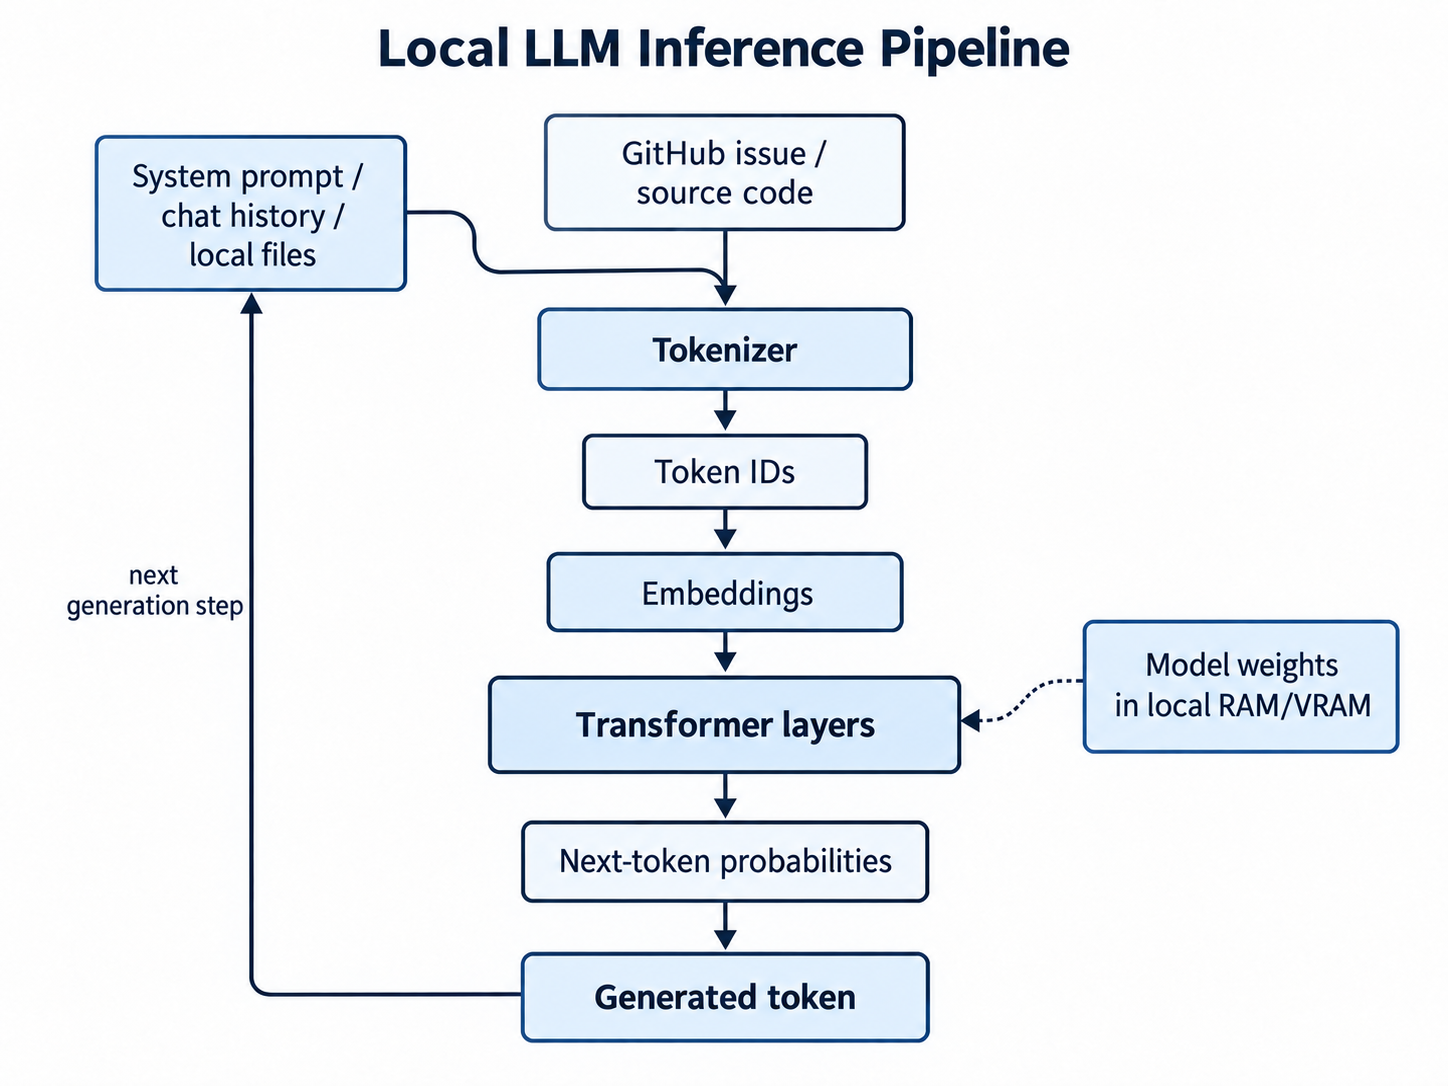
\includegraphics[width=11.5cm]{images/local-llm-inference-pipeline-autoregressive.png}
\caption{Simplified local LLM inference pipeline.}
\label{fig:local-inference-pipeline}
\end{figure}

The feedback path represents autoregressive generation: each predicted token becomes part of the context for the following step.

A model described as 8B contains approximately eight billion learned parameters, most of which are weights. These weights do not individually represent specific facts or concepts; learned information is distributed across large collections of parameters.

The number of parameters alone does not determine the memory required to store the model weights. Their numerical representation is equally important.

\section{Precision and quantization}

A useful approximation of model weight memory is
\[
M_{\text{weights}}
\approx
\frac{N_{\text{parameters}}\times b}{8},
\]
where \(b\) is the number of bits used per parameter.

FP16 uses 16 bits, or two bytes, per value. An idealised 8B model therefore requires approximately
\[
8\times 10^9 \times 2
\approx
16\text{ GB}
\]
for its weights. This calculation uses decimal gigabytes, while the model sizes in Figure~\ref{fig:llama-quantization} are reported in binary gibibytes (GiB).

Quantization reduces memory requirements by representing weights with fewer bits. In a simplified symmetric scheme,
\[
q=\operatorname{round}(w/s),
\]
where \(w\) is the original weight, \(s\) is a scale and \(q\) is a low-bit integer representation. The approximate value can later be reconstructed as
\[
\hat{w}=sq.
\]
For example, with \(s=0.1\), a weight of \(0.27\) can be stored as \(q=3\), which reconstructs to \(0.30\). This introduces quantization error. In practice, scales are typically shared by blocks of weights.

A theoretical 4-bit representation of an 8B model would require about 4 GB. Real quantization schemes also use scaling information, metadata and, in some cases, different representations for different tensors. Therefore, a scheme labelled Q4 does not imply exactly four bits per weight.

% Keep the bar chart next to its interpretation.
\noindent\begin{minipage}{\linewidth}
\centering
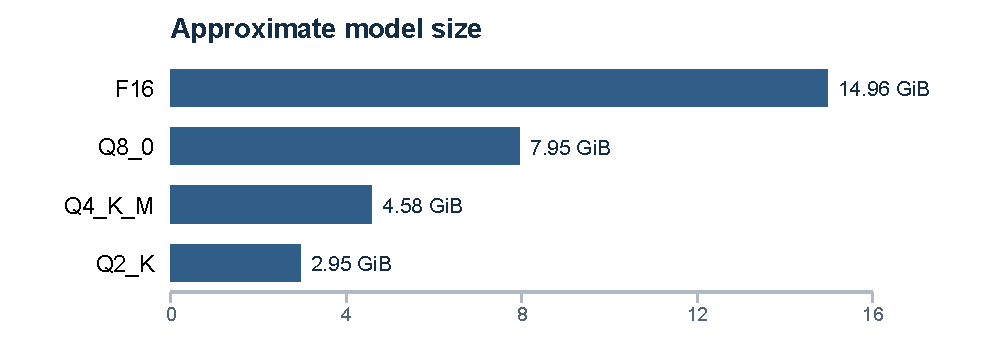
\includegraphics[width=14cm]{images/model-size-comparison.pdf}
\captionsetup{hypcap=false}
\captionof{figure}{Approximate model file sizes for different representations of Llama 3.1 8B, based on llama.cpp data \parencite{ggml-quantize}.}
\label{fig:llama-quantization}
\end{minipage}

The chart shows why quantization is useful for local deployment. \texttt{Q4\_K\_M} reduces the model file size from about 15 GiB to less than 5 GiB. The relationship between bit width and task quality is not linear: the effect depends on the model, quantization scheme and target task \parencite{ggml-quantize}.

Quantization can also improve inference speed because smaller weights reduce memory traffic. However, lower bit width does not automatically produce proportional speedups, since performance also depends on hardware support, kernels and quantization overhead.

GGUF, \texttt{Q4\_K\_M} and \texttt{llama.cpp} describe different layers of the system. GGUF is a model file format, \texttt{Q4\_K\_M} is a model quantization scheme that can use a mixture of tensor representations, and \texttt{llama.cpp} is an inference runtime that can load and execute such models \parencite{ggml-quantize,ggml-models}.

Low-precision model formats are not all equivalent. FP8 remains a floating-point representation rather than an integer-style block quantization format. Common FP8 variants include \texttt{E4M3} and \texttt{E5M2}, which trade numerical precision against dynamic range \parencite{nvidia-fp8}. Whether FP8 improves inference performance depends strongly on hardware and runtime support.

GGUF quantization names encode different quantization recipes rather than a uniform number of bits for every tensor. Common llama.cpp variants span low-bit families such as \texttt{Q2\_K}, \texttt{Q3\_K\_M}, \texttt{Q4\_K\_M}, \texttt{Q5\_K\_M} and \texttt{Q6\_K} up to \texttt{Q8\_0}. The leading number indicates the approximate precision class, while the actual effective bits per weight can differ because scales, metadata and mixed tensor representations add overhead. The K suffix identifies the K-quant family, while suffixes such as S and M distinguish smaller and medium mixed-precision variants. IQ variants, such as \texttt{IQ2\_XS} or \texttt{IQ3\_M}, use importance-aware low-bit quantization approaches. Prefixes such as UD are publisher-specific rather than core llama.cpp quantization types; Unsloth uses them for its Dynamic GGUF variants, where quantization choices may differ between layers to preserve quality \parencite{ggml-quantize,unsloth-dynamic}.

An alternative direction is to design models for extremely low-bit weights from the beginning rather than quantizing an already trained high-precision model. BitNet b1.58, for example, uses ternary weights \(\{-1,0,+1\}\), corresponding conceptually to about \(\log_2(3)\approx1.58\) bits of information per weight \parencite{ma2024bitnet}. This is a different model-design approach rather than simply another Q4-like format. Native low-bit designs can substantially reduce model-weight storage and memory-bandwidth requirements compared with conventional FP16 models. This can change the hardware cost of inference when suitable kernels and hardware support are available, although the theoretical reduction in bit width does not automatically translate into an equivalent end-to-end speedup.

\section{Runtime memory and context}

Model file size is not equal to runtime memory. A simplified model is
\[
M_{\text{runtime}}
\approx
M_{\text{weights}}
+
M_{\text{KV cache}}
+
M_{\text{temporary}}
+
M_{\text{runtime overhead}}.
\]
Therefore, a 4.6 GiB model file does not imply that 4.6 GiB of VRAM is sufficient.

For the assistant, the active context may include system instructions, a GitHub issue, repository structure, source files, previous messages, tool results and the response generated so far.

Three different context-related limits should be distinguished: the maximum context length supported by the model, the context size configured by the inference runtime, and the number of tokens actually used by a particular request. The amount of allocated KV-cache memory also depends on runtime configuration. Dynamic caches grow as more tokens are processed, while static caches may reserve capacity for a configured maximum in advance \parencite{hf-cache-strategies}.

Inference can be divided into two stages. During \textbf{prefill}, the model processes the existing context. During \textbf{decode}, it generates new tokens one by one. Transformer self-attention produces Query, Key and Value representations. Previously calculated Key and Value vectors can be stored in a \textbf{KV cache}, avoiding repeated computation during generation \parencite{hf-cache-strategies}.

The trade-off is additional memory consumption. With a dynamic cache, longer prompts, generated output and tool results appended to subsequent model requests increase the amount of active context. This is especially relevant for the assistant, which may process large source files or long test logs.

% Crop only the outer whitespace and embedded "Figure 2" caption in LaTeX.
% The original PNG is preserved unchanged; keep the diagram before its discussion.
Figure~\ref{fig:local-runtime-memory} separates model weights from the additional memory required for context and execution, explaining why model file size alone is insufficient for capacity planning.

\noindent\begin{minipage}{\linewidth}
\centering
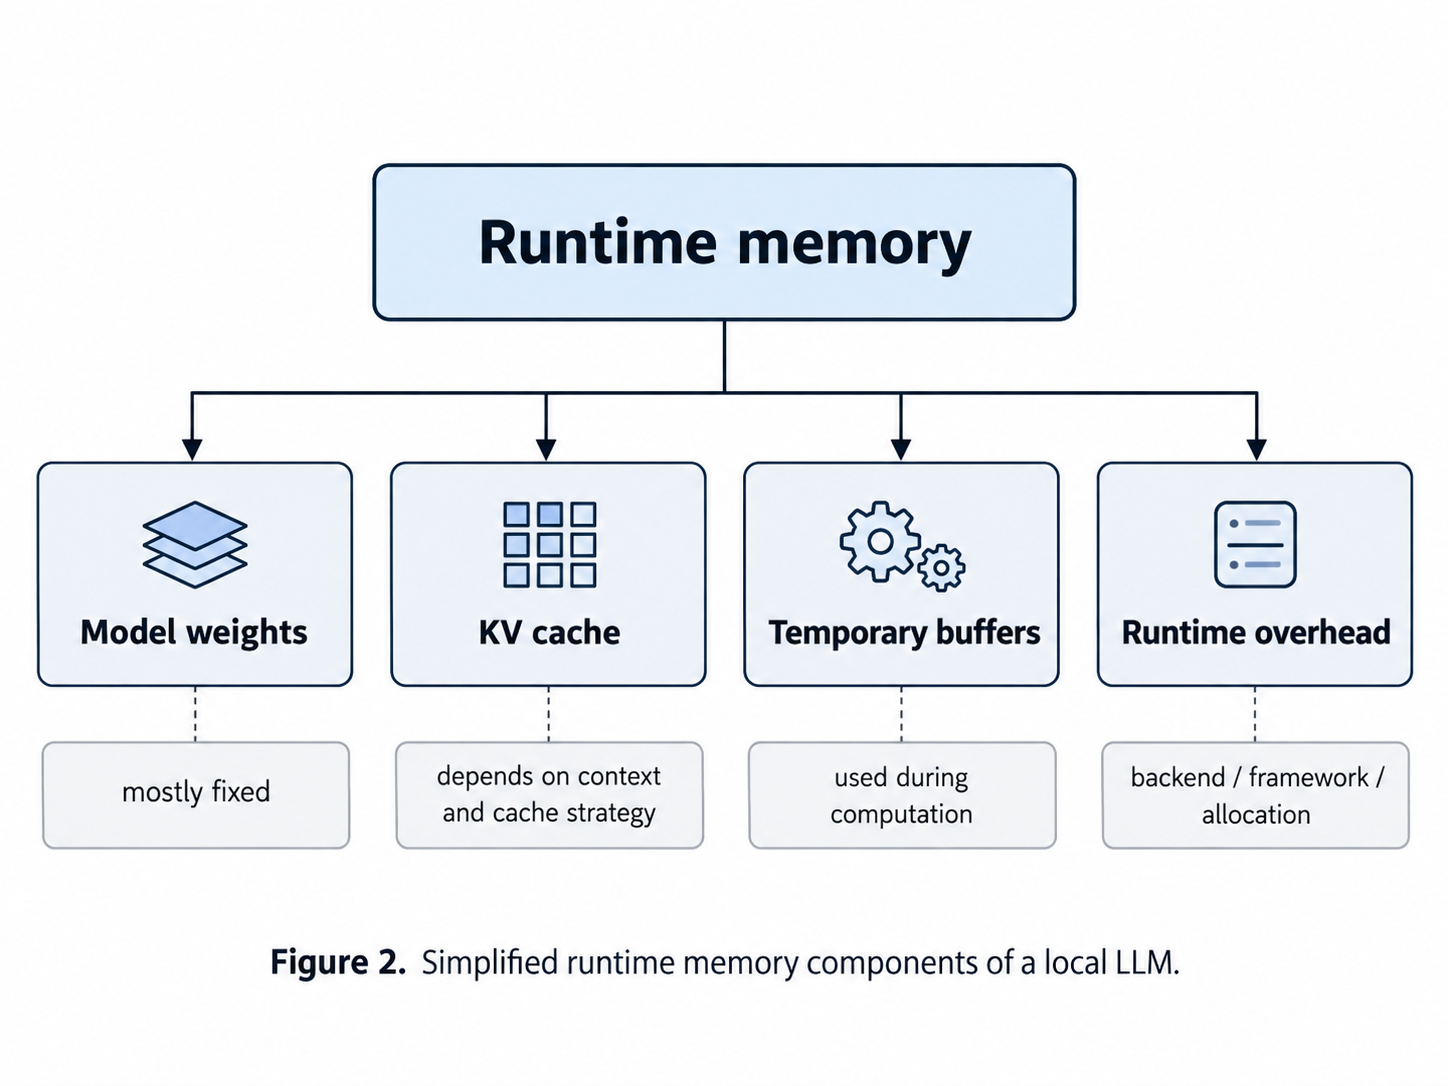
\includegraphics[width=13cm,trim=0 165bp 0 125bp,clip]{images/local-llm-runtime-memory.png}
\captionsetup{hypcap=false}
\captionof{figure}{Simplified runtime memory components of a local LLM.}
\label{fig:local-runtime-memory}
\end{minipage}

Attention architecture also affects KV-cache size. Multi-Head Attention uses many separate Key/Value heads, Multi-Query Attention uses one shared Key/Value head, and Grouped-Query Attention uses an intermediate number. Reducing the number of KV heads can lower context-memory requirements \parencite{ainslie2023gqa}.

\section{Model specialisation and deployment trade-offs}

Model specialisation is independent of quantization and local execution. A general-purpose model targets broad language tasks, while specialised models can focus on domains such as programming. Separately, instruction-tuned models are post-trained to follow user instructions effectively. A model can therefore be coding-specialised, instruction-tuned, quantized and executed locally at the same time.

For the assistant, the largest available model is not automatically the most practical choice. A smaller coding-specialised, instruction-tuned model that fits comfortably into GPU memory may be more practical to deploy than a much larger general-purpose model that requires aggressive quantization or CPU offloading.

However, practical suitability cannot be determined from parameter count or memory usage alone. Candidate models should therefore be evaluated not only on coding benchmarks, but also on their ability to follow tool-use instructions and produce changes that pass relevant tests, while remaining within the available memory, context and latency budget. These evaluation criteria lead directly to the next topic: \textbf{LLM Benchmarks and Model Selection}.

% Finish this chapter before restoring the document spacing.
\par\clearpage
\endgroup
